\section{Case Study}

\begin{frame}[allowframebreaks,fragile]
  \frametitle{Case Study}
  A language to specify a GUI to edit entities
  
  \begin{itemize}
    \item Entities
    \begin{itemize}
      \item primitive attributes
      \item derived attributes
      \item inheritance
    \end{itemize}
    \item Forms
    \begin{itemize}
      \item textboxes
      \item checkboxes
      \item validation clauses
    \end{itemize}
    
  \end{itemize}

\begin{verbatim}
entity PersonP {
	name      : string;
	firstName : string;
	age       : int; 
	weight    : float;
	likesCake : bool; 
    isAdult =  age >= 18;
	greeting = "Hello " + firstName + " " + name ;
}

entity House {
	floors : int; 
	street : string;
}

form PersonFormP1 edits PersonP {
	 text(20) -> name validate 1 == 1;
	 text(20) -> firstName validate lengthOf(firstName) > 2;
	 checkbox -> isAdult validate 1 == 1;
	 checkbox -> likesCake validate lengthOf(firstName) > 2;
}
\end{verbatim}

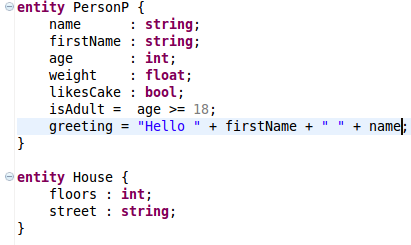
\includegraphics[width=\linewidth]{img/entities.png}

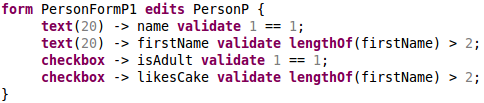
\includegraphics[width=\linewidth]{img/personform.png}

\end{frame}
